\chapter{Shiny Package Tutorial}
\section{Introductory Reading}

Shiny is a package used in R, that enables the user to easily create interactive applications.
Shiny can be used to create both simple histograms of disease data or interactive maps of the crime rate in different cities.
With Shiny the possibilities are endless.
In this lab, you will learn how to create a basic Shiny application. 
\begin{figure}
   \centering
   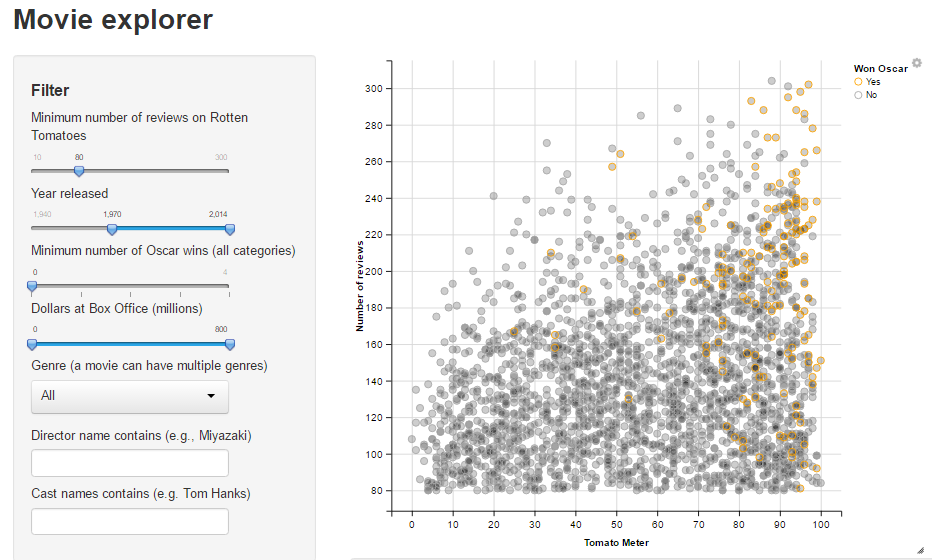
\includegraphics[width = 0.5\textwidth]{pictures/shiny/shiny.PNG} 
   \caption{Sample Shiny app}
   \label{fig:model}
\end{figure}
\noindent Look at the picture in Figure \ref{fig:model}.
\cite{gallery} This is a sample Shiny app depicting a graph of many famous movies.
The graph plots movies based on their rating and the number of reviews it has on Rotten Tomatoes.
On the left of the graph you find various inputs, such as Oscars and genres, that can customize the output of the graph.
These are the basic components of a Shiny app: inputs and outputs.     
Here are some examples of Shiny input functions:
\begin{itemize}
    \item checkboxInput: a single check box
    \item dateInput: a calendar
    \item fileInput: file upload
    \item numericInput: enter number
    \item radioButtons: set of radio buttons
    \item selectInput: box with multiple choices
    \item sliderInput: a slider bar
    \item textInput: enter text
\end{itemize}
\noindent The users of a Shiny app will interact solely with the inputs that you, the developer, will allow them to.
The above inputs can collect various types of data input from the user, to determine many different types of outputs.
Here are some of the output functions in Shiny:
\begin{itemize}
    \item imageOutput: creates image
    \item plotOutput: creates a plot
    \item tableOutput: creates a table
    \item textOutput: creates text
\end{itemize}

Understanding how inputs and outputs relate to each other is a key requirement for developing a Shiny app. In the model students will create today, the inputs will be dropdown boxes (selectInput) and the output will be a simple scatterplot (plotOutput). 

\section{Objectives}

Students will be expected to learn the basic components of a Shiny App. Students will create their own application after learning the fundamentals of the package. This application will illustrate the progression of Olympic swimming medalists' times since the modern Olympics began. 

\subsection{Objective 1}
By the end of this lesson the student will understand the various parts of a Shiny app, while building a simple population prediction application.

\subsection{Objective 2}
Students will also be able to create their own Shiny apps from scratch, and will be expected to create a Shiny app displaying Olympic swimming times over various events and years.
 
\section{Building the Model}

Shiny applications have a wide variety of uses. Today students will learn how to create a basic population prediction model. \\

\noindent To begin the application, open a new R script file in RStudio, clear the environment, set a working directory, and import the libraries necessary for this project. To clear the environment and set a directory use the following functions. Make sure you set a directory on your computer that the dataset is located in. 

\begin{lstlisting}[language = R]
rm(list=ls())
setwd("C:/Users/Ishaan/Documents/NCSSM 2015-2016")
\end{lstlisting}

\noindent The libraries are as follows:

\begin{lstlisting}[language = R]
library(ggplot2)
library(scales)
library(ggmap)
library(dplyr)
library(car)
library(gcookbook)
library(shiny)
\end{lstlisting}


\noindent If you don't have one of these libraries installed on your computer, you can simply type 
\begin{lstlisting}[language = R]
install.packages("insertlibraryname") 
\end{lstlisting}
in the console to download them. 

\noindent Next, we need to import the dataset of all the population data in NC for the next five years into a variable of your choice (I used popData).
This can be done with the read \texttt{.csv} function.
Make sure the data file is in directory you specified above. 

\begin{lstlisting}[language = R]
popData <- read.csv("Population.csv")
\end{lstlisting}
Shiny applications have two components: a user-interface definition and a server script.
The user-interface is used to control the design and layouts of the Shiny application.
The server script for the Shiny application controls the algorithms and code that tell the Shiny app how to manipulate the inputs to produce outputs.\cite{shiny} 
Three functions --- headerPanel, sidebarPanel, and mainPanel --- define the various regions of the user-interface.
The application will be called “Population Statistics” so we specify that as the title when we create the header panel.
The other panels are empty for now.
We create a UI function with the aforementioned components, like this:
\begin{lstlisting}[language = R]
ui <- shinyUI(fluidPage(
  headerPanel("Population Statistics"),
  sidebarPanel(),
  mainPanel()
))
\end{lstlisting}
Next, define a skeletal server implementation. This can be done by creating a function called server with two parameters: input and output.
\begin{lstlisting}[language = R]
server <- function(input, output) {

}
\end{lstlisting}
The server function will be empty to begin with, but it will eventually be used to set relationships between the inputs and outputs of the application. At the end of your code, we need to call the shiny function so the application will run. To do that use the following syntax: 
\begin{lstlisting}[language = R]
shinyApp(ui = ui, server = server)
\end{lstlisting}
The skeletal structure of the simplest Shiny application possible is shown in figure \ref{fig:blank}. 
Run the Shiny application by selecting all of your code and clicking the run button in the top right corner of RStudio.
The blank Shiny application should open in a new window as shown in figure \ref{fig:blank}.
\begin{figure}[h]
   \centering
   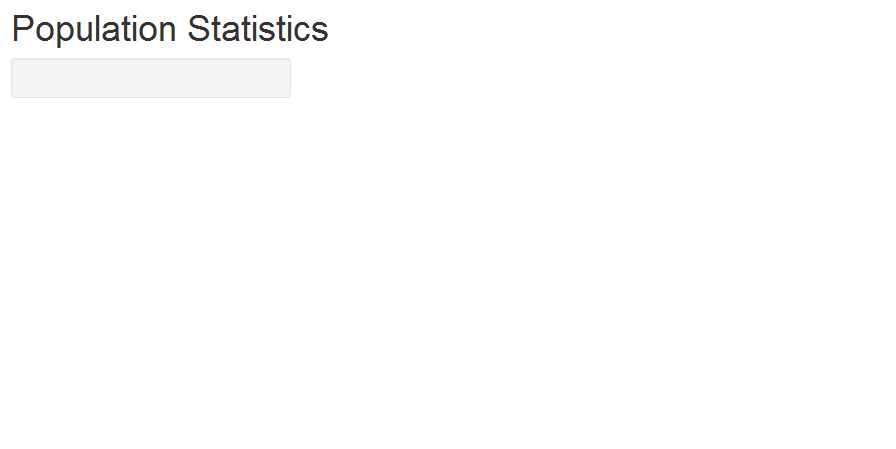
\includegraphics[width=0.5\textwidth]{pictures/shiny/blank.PNG} 
   \caption{Blank Shiny App}
   \label{fig:blank}
\end{figure}
To begin the model, we need to display the inputs of our program in the sidebar panel of the application. Our program is taking age group as an input and displaying a plot showing the predicted populations of that age group in North Carolina over the next five years. To do this, we will create a selectInput with all of the age groups as choices, like so:
\begin{lstlisting}[language = R]
sidebarPanel(
    selectInput(
        inputId = "age", 
        label = "Age:", 
        choices = c(
            "Total", "0-4 years", "5-9 years", 
            "10-14 years", "15-19 years", "20-24 years", 
            "25-29 years", "30-34 years", "35-39 years", 
            "40-44 years", "45-49 years", "50-54 years", 
            "55-59 years", "60-64 years", "65-69 years", 
            "70-74 years", "75-79 years", "80-84 years", 
            "85+ years")
    )
  )
\end{lstlisting}
The inputId is simply a name that we give to each input, so we can access them in the server function. The label is the text that will appear on the application above the input box. \\
We also need to tell the application that our plot will be displayed in the main panel of the UI. This involves creating a plotOuput, like so: 
\begin{lstlisting}[language = R]
 mainPanel(
    plotOutput(outputId = "myPlot")
 )
\end{lstlisting}
Just like in selectInput, we need to give the output an ID, so we can use that name to access it in the server function.
Once the model is run, the application should look like figure \ref{fig:drop}. 
\begin{figure}[h]
   \centering
   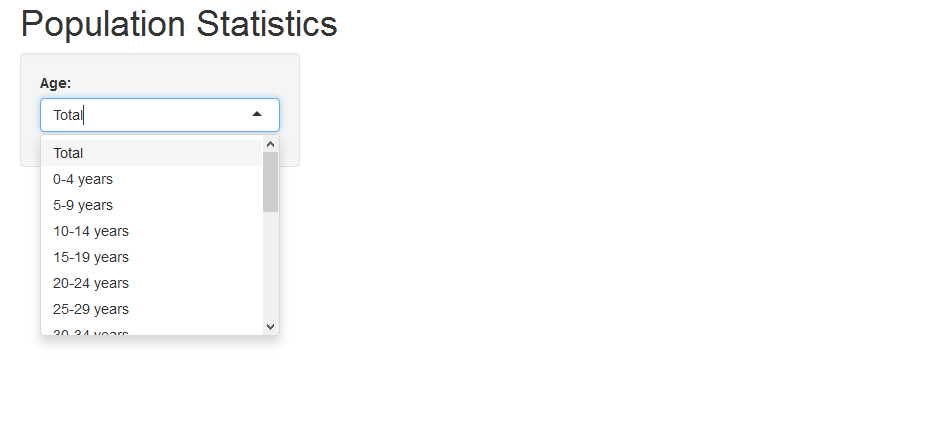
\includegraphics[width=0.5\textwidth]{pictures/shiny/dropdown.PNG} 
   \caption{Adding Inputs}
   \label{fig:drop}
\end{figure}
Next we need to define the server-side of the application which will accept inputs and compute outputs. Our server function will contain the code necessary to do this. We first tell the function that we are creating a plot as an output, and we can create the plot using the renderPlot command. The command renderPlot is what makes the application react. This means when a user changes the input, the output will instantly change. This is what makes Shiny so interactive.\\
Within the renderPlot function we first select what data we will use and then plot that data using the ggplot function. To select our data, create a variable called dataInput, and take a subset of the csv file we imported into R. We want to take only the data that the user specified, so instead of importing all the age group data, we only import the age group that the user selected. We can access that specific age group using input\$age. The ggplot function takes in various inputs, such as the data, the variables, and the title. The aes function within ggplot indicates which axis is given to which variable, while the geom\_point function draws the points on the graph. The ggtitle function creates a title over the plot. The completed server function should look like this: 
\begin{lstlisting}[language = R]
server <- function(input, output) {
  output\$myPlot <- renderPlot({
    dataInput <- subset(popData, (Age==input\$age), select=c(Year, Population, State))
    
    ggplot(
        data = dataInput, 
        aes(x=Year, y=Population)
    ) + geom_point() + ggtitle("Population")
    
 })
  
}
\end{lstlisting}
Finally, run the entire code including the shinyApp command.
Your screen should look like the screen displayed in Figure \ref{fig:example}.
The application should have a working select box, a title, and a plot displaying the population data.
\begin{figure}[h]
   \centering
   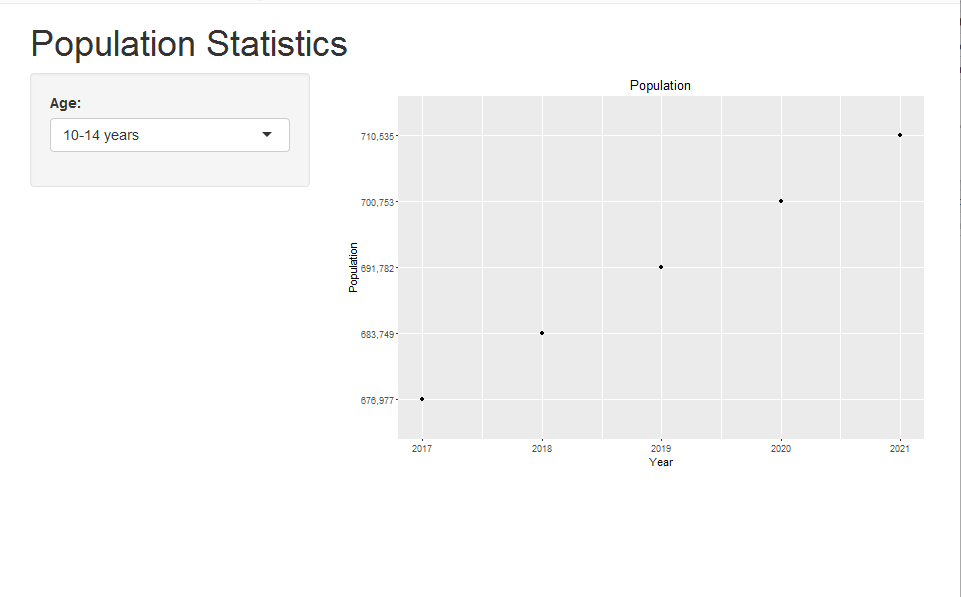
\includegraphics[width = .5\textwidth]{pictures/shiny/pop.PNG} 
   \caption{Final Model}
   \label{fig:example}
\end{figure}

\section{Deliverable}

You are expected to deliver properly formatted code written in the R language, using the Shiny package.
Additionally, you will need to provide screenshots of various input combinations to demonstrate that your application is fully functional.
This model will display Olympic swimming times over the modern Olympics.
The variables for this model include time, year, and medal.
The inputs are the event and gender of the swimmer.
The graph should display the medaling times for each event and gender for each year of the modern Olympics.
The data for this project is found within the SwimmingExampleM dataset provided. 
\subsection{Programming Hints}
 In the deliverable you will need to be able to add color to the model. It is quite simple. In the previous section we explained that the ggplot command makes the actual plot. In order to create color we just add \textbf{color =} some variable, inside the aes() function.

\begin{lstlisting}[language = R]
aes(x=Time, y=Year, color=Medal)
\end{lstlisting}
The final shiny app screen should look like figure \ref{olympic}
\begin{figure}[h]
   \centering
   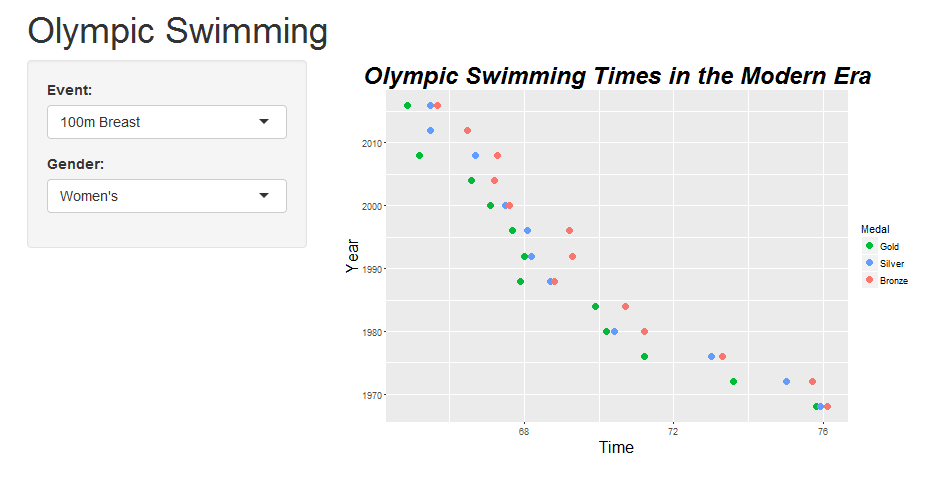
\includegraphics[width = .5\textwidth]{pictures/shiny/olympic.PNG} 
   \caption{Deliverable}
   \label{fig:olympic}
\end{figure}

\section{Teaching Code}
\begin{lstlisting}[language = R]
#Ishaan Rao
#September 1, 2016
#pop.R

#clean up and set the directory
rm(list=ls())
setwd("C:/Users/Ishaan/Documents/NCSSM 2015-2016")

#load libraries
library(ggplot2)
library(scales)
library(ggmap)
library(dplyr)
library(car)
library(gcookbook)
library(shiny)

#read data file
popData <- read.csv("Population.csv")

#setting the server, code instructing R what to do with inputs
#output\$my plot is what will be created when the app is run
#renderPlot allows Shiny to adjust when the user changes an option
#By defining the subset we indicate which inputs we want to be selected by the user
#select are the values in the dataset that are going to be plotted
#ggplot give direction to create plot, aes() defines the axes, ggtitle creates 
title and geom_point creates the scatter plot
server <- function(input, output) {
  output\$myPlot <- renderPlot({
    dataInput <- subset(popData, (Age==input\$age), select=c(Year, Population, State))
    
    ggplot(data = dataInput, aes(x=Year, y=Population)) 
    + geom_point() + ggtitle("Population")
    
  })
  
}
# Define UI for application that draws a scatterplot
#headerPanel creates the title
#sidebarPanel creates the user entered section
#selectInputs is where you insert the options that the user can select
#mainPanel outputs the app using all of the previous code we inputed
ui <- shinyUI(fluidPage(
  headerPanel("Population Statistics"),
  sidebarPanel(
    selectInput(
        inputId = "age", 
        label = "Age:", 
        choices = c(
            "Total", "0-4 years", "5-9 years", 
            "10-14 years", "15-19 years", "20-24 years", 
            "25-29 years", "30-34 years", "35-39 years", 
            "40-44 years", "45-49 years", "50-54 years", 
            "55-59 years", "60-64 years", "65-69 years", 
            "70-74 years", "75-79 years", "80-84 years", 
            "85+ years")
    )
  ),
  mainPanel(
    plotOutput(outputId = "myPlot")
  )
))
#this runs the Shiny App
shinyApp(ui = ui, server = server)

\end{lstlisting}

\section{Example Student Code}

\begin{lstlisting}[language = R]
#Ishaan Rao
#September 1, 2016
#olympic.R

#load libraries
library(ggplot2)
library(scales)
library(ggmap)
library(dplyr)
library(car)
library(gcookbook)
library(shiny)

rm(list=ls())
setwd("C:/Users/Ishaan/Documents/NCSSM 2015-2016")

swimData <- read.csv("SwimExampleM.csv")
#setting the server, code instructing R what to do with inputs
#output\$my plot is what will be created when the app is run
#renderPlot allows Shiny to adjust when the user changes an option
#By defining the subset we indicate which inputs we want to be selected by the user
#select are the values in the dataset that are going to be plotted
#ggplot give direction to create plot, aes() defines the axes, ggtitle creates 
title and geom_point creates the scatter plot
#scale_color_hue creates different colors for each of the three models\\
server <- function(input, output) {

  output\$myPlot <- renderPlot({
  
    dataInput <- subset(swimData,
             (Event==input\$event & Gender==input\$gender), 
                select=c(Time, Year, Medal, Name))
    
    ggplot(data = dataInput, aes(x=Time, y=Year, color=Medal)) + 
        geom_point(size=3) + 
        ggtitle("Olympic Swimming Times in the Modern Era") + 
        theme(
            plot.title = element_text(color="black", size=24, 
            family="Times", face="bold.italic"), axis.title = element_text(size=16)
        ) + 
        scale_color_hue(breaks=c("Gold","Silver","Bronze"))
  })
} 
# Define UI for application that draws a scatterplot
#headerPanel creates the title
#sidebarPanel creates the user entered section
#selectInputs is where you insert the options that the user can select
#In the model we have two different inputs one for event and one for gender, we 
create two different selectInput commands to account for the options
#mainPanel outputs the app using all of the previous code we inputted
ui <- shinyUI(fluidPage(
  headerPanel("Olympic Swimming"),
  sidebarPanel(
    selectInput(
        inputId = "event", 
        label = "Event:", 
        choices = c(
            "50m Free", "100m Free", "100m Back", "100m Breast", 
            "100m Butterfly", "200m Free", "200m Back", "200m Breast",
            "200m Butterfly", "200m IM", "400m IM"
        ), 
        selected = "50m Free"
    ),
    selectInput(
        inputId = "gender", 
        label = "Gender:", 
        choices = c("Men's", "Women's"),
        selected = "Women's"
    )
  ),
  mainPanel(
    plotOutput("myPlot")
  )
))
#runs application
shinyApp(ui = ui, server = server)
\end{lstlisting}


\section{Further Readings}
\begin{itemize}
\item For a full tutorial on creating a Shiny app, visit this tutorial on the Shiny website: \url{http://shiny.rstudio.com/tutorial/}.
\item To learn more advanced Shiny topics, functions, and capabilities visit: \url{http://shiny.rstudio.com/articles/}.
\item To see sample Shiny apps in action visit Shiny's gallery: \url{http://shiny.rstudio.com/gallery/}
\end{itemize}
